\chapter{Structure of a Nuclear Reactor}

When designing a power reactor core, two key criteria must be satisfied. First, criticality must be sustained across the entire range of power levels and throughout the fuel depletion process. Second, the core must allow for efficient transfer of the thermal energy produced by fission reactions without causing overheating \cite{Lewis_2014}. In this chapter, we will discuss neutron behavior and the influence of the reactor lattice on the multiplication factor.

\section{Time Dependence of Neutron Flux}
In the previous chapter, we examined neutron flux but disregarded its time dependence. To investigate this aspect, we will analyze two types of systems:

\begin{itemize}
    \item Non-multiplicative systems: Systems without fissionable material.
    \item Multiplicative systems: Systems containing fissionable material.
\end{itemize}

To perform the necessary calculations, we must define the following variables:

\begin{itemize}
    \item $n(t)$: The total number of neutrons at a given time $t$.
    \item $\bar{v}$: The average velocity of neutrons.
    \item $\Sigma_{x}$: The macroscopic cross-section for a specific reaction $x$ (e.g., absorption, scattering, or fission).
\end{itemize}

\subsection{Infinite Multiplicative Media}

In this initial approximation, we will account only for the effects of prompt neutrons and neutron leakage. Based on these assumptions, we can outline the factors contributing to the rate of change in the neutron population over time \cite{Lewis_2014}:

\begin{center}
     $\frac{d}{dt}n(t)$ = \text{neutrons produced per second by the source} \\
                     + \text{neutrons produced by fission} \\ 
                     - \text{neutrons absorbed} 
\end{center}

To represent the neutrons introduced by an external source, we define the variable \(S(t)\), which describes the rate of neutron production by the source at time \(t\) \cite{Lewis_2014}. In addition, let \(\nu\) be the average number of neutrons, thus \(\nu \Sigma_{f} \bar{v} n(t)\) is the number of fission neutrons produced per second. Finally, \(\Sigma_{a} \bar{v} n(t)\) is the number of neutrons absorbed per second. With this we get the expression:

\begin{flalign}
    && \frac{d}{dt} n(t) = S(t) + \nu \Sigma_{f} \bar{v} n(t) - \Sigma_{a} \bar{v} n(t) && 
    \label{eq:neutron_population}
\end{flalign}

It can be easily shown that the mean lifetime of a neutron, defined as the time between its production and absorption, is given by \(l_{\infty} = \frac{1}{\bar{v} \Sigma_{a}}\). By using the definition of \(k_{\infty}\) from \textbf{Eq.}(\ref{eq:infinite_multiplicative_factor}), we obtain the following equation for the time dependence of the neutron population:

\begin{equation}
    \frac{d}{dt} n(t) = S(t) + \frac{(k_{\infty} - 1)}{l_{\infty}} n(t)
    \label{eq:nt_dependence_t_kinfty}
\end{equation}

If there is no external source and neutrons are produced solely through fission (\(S(t) = 0\)), the equation simplifies to:

\begin{equation*}
    \frac{d}{dt} n(t) = \frac{(k_{\infty} - 1)}{l_{\infty}} n(t)
\end{equation*}

This equation describes three possible behaviors for the neutron population, depending on the value of \(k_{\infty}\):

\begin{itemize}
    \item \(k_{\infty} < 1\): The neutron population decreases exponentially, indicating a sub critical state.
    \item \(k_{\infty} > 1\): The neutron population increases exponentially, corresponding to a supercritical state.
    \item \(k_{\infty} = 1\): The neutron population remains constant, representing a critical state.
\end{itemize}

\subsection{Finite Multiplicative Media}

In real life nuclear reactors are finite, thus neutrons could escape through the borders of the reactor. This effect should be considered in the rate of change in the neutrons populations:

\begin{center}
    $\frac{d}{dt}n(t)$= \text{neutrons produced per second by the source} \\
    + \text{neutrons produced by fission} \\ 
    - \text{neutrons absorbed} \\
    - \text{neutrons escaping the system} 
\end{center}

First, it is important to notice that the effect of the leakage of neutrons is proportional to neutrons population at a time t \cite{Lewis_2014}. Define the coefficient \(\Gamma\) in a way that:

\begin{flalign*}
   && \text{Neutrons escaping the system} = \Gamma \Sigma_{a} \bar{v} n(t) &&
\end{flalign*}

This leads to:

\begin{flalign}
   && \frac{d}{dt}n(t) = S(t) + \nu \Sigma_{f} \bar{v} n(t) - \Sigma_{a} \bar{v} n(t) - \Gamma \Sigma_{a} \bar{v}n(t) &&
   \label{eq:n_population_leakage}
\end{flalign}

From the definition of \(\Gamma\), we can deduce expressions for the leakage probability (\(P_{L}\)) and the non-leakage probability (\(P_{NL}\)). The non-leakage probability corresponds to neutrons that remain inside the reactor and can induce new fissions. We define the leakage probability as:

\begin{flalign*}
    P_{L} = \frac{\text{neutrons that escape}}{\text{neutrons produced}}
\end{flalign*}


which gives the following expression \cite{Lewis_2014}:

\begin{flalign*}
   && P_{L} = \frac{\Gamma \Sigma_{a} \bar{v} n}{\Sigma_{a} \bar{v} n + \Gamma \Sigma_{a} \bar{v} n} = \frac{\Gamma}{1 + \Gamma} &&
\end{flalign*}

The non-leakage probability \(P_{NL}\) can be easily derived from the definition of \(P_{L}\) as:

\begin{flalign}
   && P_{NL} = \frac{1}{1 + \Gamma} &&
\end{flalign}

In the next section, we will explore the relationship between the size and shape of the reactor and the parameter \(\Gamma\). For now, we can rewrite \textbf{Eq.}(\ref{eq:n_population_leakage}) in terms of \(P_{NL}\) as follows:

\begin{flalign*}
   && P_{NL} \frac{d}{dt}n(t) = P_{NL}S(t) + \frac{(P_{NL}k_{\infty}-1)}{l_{\infty}} n(t) &&
\end{flalign*}

By defining \(k = k_{\infty}P_{NL}\) and \(l = l_{\infty}P_{NL}\), and substituting these into the above equation, we obtain:

\begin{flalign}
    && \frac{d}{dt}n(t) = S(t) + \frac{(k-1)}{l} n(t) &&
\end{flalign}

\subsection{Delayed Neutron Kinetics}

Around \(99 \, \%\) of fission neutrons are prompt neutrons, emitted at the moment of fission \cite{Lewis_2014}. The remaining fraction, denoted by \(\beta\), are delayed neutrons emitted through the decay of fission products. The nuclei that emit the delayed neutrons are divided in six groups based on their half-lives, which go from a fraction of a second to nearly a minute  \cite{Lewis_2014}. These groups are showed in the Table \ref{tb:delayed_neutrons_fraction}.

\begin{table}[h]
    \caption{Delayed Neutron Fractions for Different Isotopes. From \textbf{Ref.} \cite{Lewis_2014}}
    \centering
    \begin{tabular}{lccc}
        \toprule
        Approximate Half-life (sec) & U\textsuperscript{233} & U\textsuperscript{235} & Pu\textsuperscript{239} \\
        \midrule
        56   & 0.00023 & 0.00021 & 0.00007 \\
        23   & 0.00078 & 0.00142 & 0.00063 \\
        6.2  & 0.00064 & 0.00128 & 0.00044 \\
        2.3  & 0.00074 & 0.00257 & 0.00069 \\
        0.61 & 0.00014 & 0.00075 & 0.00018 \\
        0.23 & 0.00008 & 0.00027 & 0.00009 \\
        \midrule
        Total delayed fraction & 0.00261 & 0.00650 & 0.00210 \\
        Total neutrons/fission & 2.50    & 2.43    & 2.90    \\
        \bottomrule
    \end{tabular}
    \label{tb:delayed_neutrons_fraction}
\end{table}

We defined \(\beta\) as the sum of the delayed neutron fraction of each group, this is:

\begin{equation}
    \beta = \sum_{i=1}^{6}\beta_{i}
\end{equation}

For instance, consider the half-life for the \(i\)th group, \(t_{i1/2}\). Using these half-lives we can define the average half-life of the delayed neutrons by :

\begin{equation*}
    t_{1/2} = \frac{1}{\beta} \sum_{i=1}^{6} \beta_{i} t_{i1/2}
\end{equation*}

Since half-lives and decay constant are related by \(t_{i1/2} = \left. 0.693 \right/ \lambda_{i}\), it is possible to define the average decay constant by :

\begin{equation}
    \frac{1}{\lambda} =  \frac{1}{\beta} \sum_{i=1}^{6}\beta_{i}\frac{1}{\lambda_{i}}
\end{equation}

Until now, the mean lifetimes \(l\) and \(l_{\infty}\) have only included the contribution of prompt neutrons. To account for the contributions of delayed neutrons, denoted by \(l_{d}\), we must derive an expression for their lifetime:

\begin{flalign}
    l_{d} = \underbrace{l}_{\text{Term 1}} + \underbrace{\frac{1}{\lambda}}_{\text{Term 2}}
\end{flalign}

The first term represents the time it takes for a delayed neutron to be absorbed or to escape, while the second term accounts for the time between the fission of the parent nucleus and the emission of the delayed neutrons through the decay of fission products.

Taking both, prompt and delayed neutrons, into account, the average neutron lifetime is defined as:

\begin{flalign}
    \bar{l} = (1 - \beta)l + \beta l_{d} = l + \frac{\beta}{\lambda}
\end{flalign}

It is clear that \(\bar{l} >> l\). The presence of delayed neutrons significantly increases the mean neutron lifetime, leading to modifications to the equations for the rate of change in neutron population, such as equation (\ref{eq:n_population_leakage}), due to the substantial delays involved.

\subsection{Kinetic Equations}

To incorporate the effects of delayed neutrons into the neutron balance equation (\ref{eq:n_population_leakage}), we separate the contributions from prompt and delayed neutrons. Defining the fraction of delayed neutrons as \(\beta\), the prompt neutrons are produced at a rate \((1-\beta) \nu \Sigma_{f} \bar{v} n(t)\) \cite{Lewis_2014}. The delayed neutrons, on the other hand, are produced by the decay of fission products. Let \(C_{i}(t)\) represent the number of precursor nuclei producing neutrons with a half-life \(t_{i1/2}\). Thus, the production rate of delayed neutrons is \(\lambda_{i}C_{i}(t)\). The resulting expression for the neutron population balance is as follows:

\begin{flalign}
    && \frac{d}{dt}n(t) = S(t) + (1-\beta) \nu \Sigma_{f} \bar{v} n(t) + \sum_{i} \lambda_{i}C_{i}(t) - \Sigma_{a} \bar{v} n(t) - \Gamma \bar{v} n(t) &&
    \label{eq:kinetic_eq_1}
\end{flalign}

Since the concentration of the precursors is unknown, we require extra equations to determine their concentrations. We divided the delayed group in six subgroups we are going to have six different equations, each one with the form of a balance equation \cite{Lewis_2014}:

\begin{flalign*}
    && \frac{d}{dt}C_{i}(t) = \text{precursors produced per second} - \text{precursors decaying per second} &&
\end{flalign*}

The number of precursors produced per second is \(\beta_{i} \nu \Sigma_{f} \bar{v} n(t)\) while the decay rate is \(\lambda_{i}C_{i}(t)\). This leads to:

\begin{flalign}
    && \frac{d}{dt}C_{i}(t) = \beta_{i} \nu \Sigma_{f} \bar{v} n(t) - \lambda_{i} C_{i} \qquad i = 1, 2, 3, ... ,6 &&
    \label{eq:kinetic_eq_2}
\end{flalign}

\subsubsection{Reactivity}

The reactivity is defined:

\begin{flalign}
    \rho = \frac{k - 1}{k}
    \label{eq:def_reactivity}
\end{flalign}

The reactivity can have three possible conditions:

\begin{flalign*}
    \rho =
    \begin{cases}
        > 0 & \text{(supercritical)} \\
        = 0 & \text{(critical)} \\
        < 0 & \text{(subcritical)}
    \end{cases}
\end{flalign*}

Additionally, define the prompt generation time as \(\Lambda = \left. 1 \right/ k\) with these definitions the kinetics equations (\ref{eq:kinetic_eq_1}) and (\ref{eq:kinetic_eq_2}) can be simplified as:

\begin{flalign}
    && \frac{d}{dt}n(t) = S(t) + \frac{(\rho-\beta)}{\Lambda} n(t) + \sum_{i} \lambda_{i}C_{i}(t) && \\
    && \frac{d}{dt}C_{i}(t) = \frac{\beta_{i}}{\Lambda}n(t) - \lambda_{i}C_{i}(t), \qquad i = 1,2, \dotsc, 6 &&
\end{flalign}

\section{Spatial Diffusion of Neutrons}

We have included the diffusion of neutrons by introducing the factor \(P_{NL}\). However, a better understanding of the relation between \(P_{NL}\) and the shape and size of a nuclear reactor is necessary to understand how these parameters affects the reactivity.

\subsection{Continuity Equation}

Consider an arbitrary volume \(V\), centered at \(\Vec{r} = (x, y, z)\), and establish a balance equation between the number of neutrons leaving and entering \(V\) \cite{Lamarsh_Baratta_2009}:

\begin{flalign*}
    \text{Neutrons leaking from } V + \text{ Neutrons absorbed inside } V = && \\ 
   \text{Neutrons emitted by a source inside } V \\ 
   + \text{ Neutrons produced by fission inside } V
\end{flalign*}

\subsubsection{Neutron Leaking}

Neutrons pass through the surface of the volume. To describe this, we define \(\Vec{J} = J(x, y, z)\) as the current density per \(cm^{2}\). If \(J_{i}\) represents the neutron current along the \(j-k\) plane, then:

\begin{flalign*}
    && \textbf{Neutron leaking} = \sum_{i=x}^{z} \left[ J_{i}\left(i + \frac{1}{2} di, \dotsb\right) - J_{i}\left(i - \frac{1}{2} di, \dotsb\right) \right] \frac{1}{di} &&
\end{flalign*}

This can be expressed as:

\begin{flalign}
    && \textbf{Neutron leaking} = \int_{V} (\nabla \cdot \Vec{J}) \, dV &&
\end{flalign}

\subsubsection{Neutrons Absorbed}

The number of neutrons absorbed is given by \(\Sigma_{a} \Phi\) \cite{Lamarsh_Baratta_2009}, where \(\Phi\) is the neutron flux defined as \(\Phi = \bar{v}n'''\). Thus:

\begin{flalign}
   && \textbf{Neutrons absorbed} = \int_{V} \Sigma_{a} \Phi \, dV &&
\end{flalign}

Here, \(n'''\) is averaged over all energy ranges: \(\bar{n'''} = \int_{0}^{\infty} n'''(E) \, dE\). Additionally, \(\Phi = \Phi(E,\Vec{r})\) can be expressed as \(\phi(\Vec{r}) = \int_{0}^{\infty} \phi(E, \Vec{r}) dE\) with this change the flux depends on \(\Vec{r}\) \cite{Lamarsh_Baratta_2009}.

\subsubsection{Neutrons Produced by a Source}

Let \(S'''(\Vec{r})\) represent the number of neutrons produced by a source per second per unit volume. The total number of neutrons produced inside \(V\) is:

\begin{flalign}
   && \textbf{Neutrons produced by a source} = \int_{V} S''' \, dV &&
\end{flalign}

\subsubsection{Neutrons Produced by Fission}

The total number of neutrons produced by fission inside \(V\) is given by:

\begin{flalign}
    && \textbf{Neutrons produced by fission} = \int_{V} \nu \Sigma_{f} \Phi \, dV &&
\end{flalign}

\subsubsection{Balance Equation}

Since all the terms introduced are integrated over the same volume, the integral over volume can be removed. In a stationary state, where the neutron population remains constant over time (\(\partial n / \partial t = 0\)), the continuity equation becomes:

\begin{flalign}
    && \nabla \cdot \Vec{J} + \Sigma_{a}(\Vec{r}) \phi(\Vec{r}) = S'''(\Vec{r}) + \nu \Sigma_{f}(\Vec{r}) \phi(\Vec{r}) &&
    \label{eq:Balance_equaitom}
\end{flalign}

However, in the equation we got two unknowns variables, \(\Vec{J}\) and \(\phi\), this forces us to express \(\nabla \cdot \Vec{J}\) in terms of \(\phi\). In order to solve this situation, we will use the diffusion approximation and the Fick's Law \cite{Lamarsh_Baratta_2009}.

\subsection{Diffusion approximation}

Fick's law is the start point of diffusion theory \cite{Lamarsh_Baratta_2009}. Fick's law states that if the concentration of a solute is grater in one region of a solution than in another, the solute diffuses from the region of higher concentration to the region of lower concentration. Moreover, the rate of solute flow is proportional to the negative of the gradient of the solute concentration \cite{Lamarsh_Baratta_2009}. A good approximation is to assume that neutrons inside a reactor behave mostly as a solute in a solution, this is:

\begin{flalign}
    \Vec{J} = -D(\Vec{r})\nabla\phi
    \label{eq:Ficks_law}
\end{flalign}

Where D denotes the diffusion coefficient. In an approximation, \(D(\Vec{r}) = \left. 1\right/ 3\Sigma_{tr} \), where \(\Sigma_{tr}\) is the transport cross sections, defined as \(\Sigma_{tr} = \Sigma_{t} - \bar{\mu}\Sigma_{s}\), where \(\bar{\mu}\) is the average scattering angle. For isotropic scattering, \(\bar{\mu} = 0\). This reduces the transport cross section to the total cross section \(\Sigma_{t}\) \cite{Lewis_2014}.

Using Fick's law in \textbf{Eq.}(\ref{eq:Balance_equaitom}) one gets the neutron diffusion equation \cite{Lewis_2014}:

\begin{flalign}
    && - \nabla \cdot D(\Vec{r})\nabla\phi + \Sigma_{a}(\Vec{r}) \phi(\Vec{r}) = S'''(\Vec{r}) + \nu \Sigma_{f}(\Vec{r}) \phi(\Vec{r}) &&
    \label{eq:diffusion_equation}
\end{flalign}

\subsection{Boundary Conditions}

It is easy to notice that the diffusion equation is a second order equation. This means that, for example, in one dimensional problems, two arbitrary constants are part of the solution. In order to know the value of these constants two boundary conditions must be known. An easy way to determinate these conditions is to use what is known as partial currents \cite{Lewis_2014}. To understand the partial currents, let \(J_{x}(x)\) be the net number of neutrons crossing the plane \(y-z\) per second per \(cm^{2}\). Now we factorize \(J_{x}(x)\) in two different contributions: \(J_{x}^{+}(x)\) and \(J_{x}^{-}(x)\) traveling in the positive and negative x directions, respectively \cite{Lewis_2014}. Then:

\begin{flalign*}
    && J_{x} = J_{x}^{+}(x) - J_{x}^{-}(x) &&
\end{flalign*}

It  can be shown that in the diffusion approximation:

\begin{flalign*}
    && J_{x}^{\pm}(x) = \frac{1}{4} \phi(x) \pm \frac{1}{2} J_{x}(x) &&
\end{flalign*}

Employing \textbf{Eq.}(\ref{eq:Ficks_law}) the equation yields:

\begin{flalign*}
    && J_{x}^{\pm}(x) = \frac{1}{4} \phi(x) \pm \frac{1}{2} D(r)\frac{d}{dx}\phi(x) &&
\end{flalign*}

We can define the boundaries of this surface as \(x_{r}\) and \(x_{l}\). In this case we, imagine a surface that does not allow any neutrons to enter, which could occur if a vacuum extends infinitely without any neutron sources. This scenario is known as a vacuum boundary condition.

If the boundary is located at \(x_{l}\), the neutron current condition can be expressed as \(J_{x}^{+}(x_{l})=0\). Conversely, for a boundary at \(x_{r}\), the condition would be \(J_{x}^{-}(x_{r})=0\). Using the definition of the partial current, we can write the condition for the right boundary as:

\begin{flalign*}
    && 0 = \frac{1}{4} \phi(x_{r}) - \frac{1}{2}D\left|\frac{d}{dx}\phi(x)\right|_{x_{r}}&&
\end{flalign*}

Furthermore, in the context of isotropic scattering, the diffusion coefficient is defined as \(D=\frac{1}{3\Sigma_{t}}\), while the mean free path \(\lambda\) is given by \(\lambda=\frac{1}{\Sigma_{t}}\). This allows us to reformulate the vacuum boundary condition as:

\begin{flalign*}
    && \frac{\phi(x_{r})}{\left|\frac{d}{dx}\phi(x)\right|_{x_{r}}} = \frac{2}{3} \lambda &&
\end{flalign*}

Let \(d = \frac{2}{3}\lambda \approx 0.66 \lambda\). Frequently, when vacuum boundaries are encountered, the most straightforward approach is to apply the zero-flux condition and adjust the dimensions accordingly. This is expressed as \(\phi(x_{r} + d) = 0\) and \(\phi(x_{l} + d) = 0\). We refer to these conditions as the extrapolated boundaries, denoted by \(\Tilde{x_{r}}\) and \(\Tilde{x_{l}}\). 

A more accurate approach, based on transport theory, yields a value of \(d_{tr} = 0.7104 \lambda\). This concept is illustrated in \textbf{Fig} \ref{fig:extrapolated_bc}.

\begin{figure}[h]
    \centering
    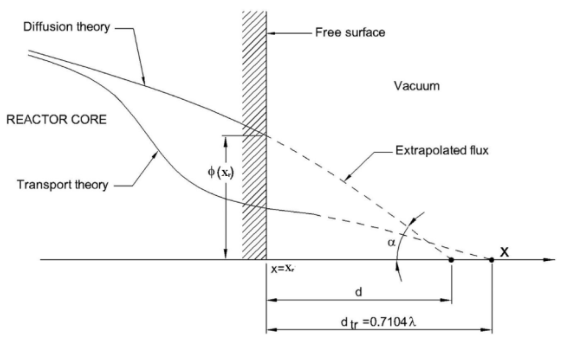
\includegraphics[width=0.75\linewidth]{Kap4/Figures_Kap4/extrapolated_bc_edit_2.png}
    \caption{Extrapolated boundary conditions. From \textbf{Ref.} \cite{book_science_direct}}
    \label{fig:extrapolated_bc}
\end{figure}

\section{Non-Leakage Probability}

Finally, to determinate the non-leakage probability lets consider a multiplicative (\(\nu\Sigma_{f} > 0\)) and uniform system, which means that the source \(S'''(r) = S_{0}'''\), \(D(\Vec{r}) = D = cte\) and all cross section are space-independent constants. Additionally, let \(L = \sqrt{D/\Sigma_{a}}\) and take \(k_{\infty}\) as defined in \textbf{Eq.}(\ref{eq:def_infty_sigmas}). Including all of these in the diffusion equation (\ref{eq:diffusion_equation}) we get:

\begin{flalign}
    && - \nabla^{2} \phi(\Vec{r}) + \frac{1}{L^{2}} \phi(\Vec{r}) = \frac{1}{D}s_{0}''' + \frac{1}{L^{2}}k_{\infty}\phi(\Vec{r}) &&
    \label{eq:std_diffusion}
\end{flalign}

\subsection{Spherical Geometry}

In spherical geometry, the Laplacian \(\nabla^{2}\) is replaced by:

\begin{flalign*}
    && - \frac{1}{r^{2}} \frac{d}{dr}\left( r^{2} \frac{d\phi}{dr} \right) + \frac{1}{L^{2}} (1 - k_{\infty}) \phi = \frac{1}{D} S_{0}''' &&
\end{flalign*}

The solution to this equation is a superposition of the general and particular solutions, \(\phi(r) = \phi_{g}(r) + \phi_{p}(r)\). Assuming a uniform source, we have \(\phi_{p}(r) = \text{const} = \frac{S_{0}'''}{(1 - k_{\infty}) \Sigma_{a}}\) \cite{Lewis_2014}.

For the general solution, consider the case where \(k_{\infty} < 1\). The equation becomes:

\begin{flalign*}
    && \frac{1}{r^{2}} \frac{d}{dr} \left( r^{2} \frac{d\phi_{g}}{dr} \right) - \frac{1}{L^{2}} (1 - k_{\infty}) \phi_{g} = 0 &&
\end{flalign*}

Applying the previously discussed boundary conditions, the solution is:

\begin{flalign*}
    && \phi(r) = \frac{S_{0}'''}{(1 - k_{\infty}) \Sigma_{a}} \left[ 1 - \frac{\Tilde{R} \sinh(\kappa r)}{r \sinh(\kappa \Tilde{R})} \right] &&
\end{flalign*}

where \(\kappa = \frac{1}{L} \sqrt{1 - k_{\infty}}\) and \(\Tilde{R} = R + \frac{2}{3} \lambda\), representing the extrapolated boundary conditions.

Now consider the supercritical case \(k_{\infty} > 1\), where the particular solution is:

\begin{flalign*}
    && \phi_{p} = - \frac{S_{0}'''}{(k_{\infty} - 1)\Sigma_{a}} &&
\end{flalign*}

Solving the general equation and applying the boundary conditions, the solution is:

\begin{flalign*}
    && \phi(r) = \frac{S_{0}'''}{(k_{\infty} - 1)\Sigma_{a}} \left[ \frac{\Tilde{R} \sin(Br)}{r \sin(B \Tilde{R})} - 1 \right] &&
\end{flalign*}

where \(B = \frac{1}{L} \sqrt{k_{\infty} - 1}\).

\subsubsection{Criticality Condition}

In the supercritical solution, consider the limit \(B\Tilde{R} \rightarrow \pi \) then \( \phi_{p} \rightarrow \infty\), implying that the sphere becomes critical \cite{Lewis_2014}. The condition for criticality is then:

\[
\frac{1}{L} \sqrt{k_{\infty} - 1} \Tilde{R} = \pi
\]

Solving for \(k_{\infty}\) gives:

\[
k_{\infty} = 1 + \frac{\pi^{2} L^{2}}{\Tilde{R}^{2}}
\]

For a finite reactor, the criticality condition is \(k = P_{NL} k_{\infty} = 1\). Thus, for the critical sphere, the non-leakage probability is:

\begin{flalign}
    && P_{NL} = \frac{1}{1 + \left( \frac{\pi L}{\Tilde{R}} \right)^2} &&
\end{flalign}

Now lets define two new variables. First, the material buckling defined as \(B_{m} = \frac{1}{L}\sqrt{k_{\infty-1}}\) and secondly the geometrical buckling \(B_{g} = \pi/\Tilde{R}\). With this the criticality condition can be expressed as:

\begin{flalign*}
    && B_{m} = B_{g} &&
\end{flalign*}

\subsection{Time-Independent Diffusion Equation}

If we set the source to be zero, then the steady diffusion equation (\ref{eq:diffusion_equation}) becomes:

\begin{flalign}
    && \nabla \cdot D(\Vec{r})\nabla\phi(\Vec{r}) + \nu \Sigma_{f}\phi(\Vec{r}) - \Sigma_{a}\phi(\Vec{r}) = 0 &&
    \label{eq:time_ind_diffusion}
\end{flalign}

In this equation, \(\phi\) tends to zero if the reactor is subcritical. Conversely, if the reactor is in a supercritical state, \(\phi\) tends to infinity. In either case, the kinetic equations (\ref{eq:kinetic_eq_1}) and (\ref{eq:kinetic_eq_2}) are necessary to describe the system's behavior \cite{Lewis_2014}. The challenge is to determine the critical state by varying the reactor's geometry or its material composition \cite{Lewis_2014}. 

To compute this, we apply the following approach: suppose it is possible to adjust the average number of neutrons produced per fission (\(\nu\)) by a factor \(\nu_{0}/\nu\), where \(\nu_{0}\) is the number of neutrons per fission required to bring the reactor to a critical state \cite{Lewis_2014}. Since \(k \sim \nu\), we have \(\nu_{0}/\nu = 1/k\) \cite{Lewis_2014}. Thus, the time-independent diffusion equation (\ref{eq:time_ind_diffusion}) can be rewritten as:

\begin{flalign}
    && \nabla \cdot D(\Vec{r}) \nabla \phi(\Vec{r}) + \frac{1}{k} \nu \Sigma_{f} \phi(\Vec{r}) - \Sigma_{a} \phi(\Vec{r}) = 0 &&
    \label{eq:eigen_diffusion_equation}
\end{flalign}

It is easy to see that if \(\nu_{0} > \nu\), then the reactor is subcritical. On the other hand, if \(\nu_{0} < \nu\), the reactor is supercritical. By incorporating this adjustment into the diffusion equation and solving for \(k\), we transform the problem into finding how far a given configuration (defined by the reactor core's dimensions and cross-sections) is from criticality. 

This can be framed as an eigenvalue problem, where \(k\) is the eigenvalue and \(\phi\) is the eigenfunction. Typically, these problems have an infinite set of solutions. However, by applying the boundary conditions and focusing on physically meaningful solutions, those in which the neutron flux is positive everywhere within the reactor, we narrow the problem to the relevant solution. This solution corresponds to the largest eigenvalue, the corresponding eigenfuntion \(\phi\) is refered as the fundamental mode solution.

\subsubsection{Uniform Reactors}

Now suppose that the reactor is uniform, which implies that \(D\) is constant. Using the same definitions for \(k_{\infty}\) and \(L^{2}\) as in equation (\ref{eq:std_diffusion}), the diffusion equation (\ref{eq:eigen_diffusion_equation}) can be written as:

\begin{flalign*}
    && \nabla^{2}\phi + \frac{k_{\infty}/k - 1}{L^{2}} \phi = 0 &&
\end{flalign*}

Since the term multiplying \(\phi\) is constant, we define \(B^{2} = \frac{k_{\infty}/k - 1}{L^{2}}\). From this equation, it can be shown that the non-leakage probability \(P_{NL}\) is:

\[
P_{NL} = \frac{1}{1 + (LB)^{2}}
\]

Here, \(B\) is referred to as the geometric buckling, or simply the buckling \cite{Lewis_2014}. To determine the buckling, we must solve the following equation, which is the Helmholtz equation:

\begin{flalign}
    && \nabla^{2}\phi + B^{2} \phi = 0 &&
    \label{eq:helmholtz_buckling}
\end{flalign}

The solution must satisfy the condition \(0 < \phi < \infty\) within the reactor, as well as the boundary conditions at the reactor's surfaces \cite{Lewis_2014}.


\subsection{Cylindrical Reactor}

Given a cylindrical reactor with an extrapolated radius \(\Tilde{R} = R + \frac{2}{3} \lambda\) and height \(\Tilde{H} = H + \frac{4}{3} \lambda\), we now examine the buckling. Replacing \(\nabla^2\) in equation (\ref{eq:helmholtz_buckling}) with its form in cylindrical coordinates gives:

\begin{flalign*}
    && \frac{1}{r}\frac{\partial}{\partial r} \left( r\frac{d\phi}{dr} \right) + \frac{\partial^{2}}{\partial z^{2}} \phi + B^{2}\phi = 0 &&
\end{flalign*}

This equation corresponds to a partial differential equation that can be solved by separating variables. Assuming the solution takes the form \(\phi(r, z) = \psi(r) \chi(z)\), substituting and dividing by \(\phi\) yields:

\begin{flalign*}
    && \frac{1}{\psi} \frac{d}{dr} \left( r\frac{d\psi}{dr} \right) + \frac{1}{\chi} \frac{d^{2}\chi}{dz^{2}} + B^{2} = 0 &&
\end{flalign*}

Since \(B^{2}\) is a constant, the first term depends only on \(r\), and the second term depends only on \(z\), meaning each term must equal a constant for the equation to have a solution. Thus, we assume that the total buckling can be written as \(B_{r}^{2} + B_{z}^{2} = B^{2}\). These constants must satisfy the following differential equations:

\begin{flalign*}
    && \frac{d}{dr}\left( r\frac{d\psi}{dr} \right) + B_{r}^{2} \psi = 0 && \\
    && \frac{d^{2}\chi}{dz^{2}} + B_{z}^{2} \chi = 0 &&
\end{flalign*}

Solving these equations gives the expressions \(B_{z} = \pi/\Tilde{H}\) and \(B_{r} = 2.405/\Tilde{R}\). Thus, the total buckling is:

\begin{flalign}
    B^{2} = \left( \frac{2.405}{\Tilde{R}} \right)^{2} + \left( \frac{\pi}{\Tilde{H}} \right)^{2}
    \label{eq:cylindrical_buckling}
\end{flalign}

Although spherical reactors are the most efficient due to their higher non-leakage probability (\(P_{NL}\)), they represent significant technical challenges, such as structural complexity and cooling issues \cite{Notas_sanabricas}. This is why most commercial reactors have cylindrical geometry. 

In the next chapter, we will explore the different fuels used in reactors, examining how they are managed before, during, and after reactor operation.
